%%%%%%%%%%%%%%%%%%%%%%%%%%%%%%%%%%%%%%
  %%%%%%%%%%%%%%%%%%%%%%%%%%%%%%%%%%%%%%
  % Do not edit the TeX file your work
% will be overwritten.  Edit the RnW
% file instead.
%%%%%%%%%%%%%%%%%%%%%%%%%%%%%%%%%%%%%%
  %%%%%%%%%%%%%%%%%%%%%%%%%%%%%%%%%%%%%%
  
  
      
Our final data analysis example is an application of population genetics. 
Given a database of individuals and their genotypes at selected genetic loci, 
population geneticists often seek identify the presence of latent populations, 
infer the populuation of origin for specific loci, 
and estimate the degree to which populations are admixed in each individual. 
Identifying admixed individuals and characterizing latent populations 
give clues to understanding ancestral migration patterns. 

The data we use come from a study of 155 samples of an endangered bird species, the Taita thrush CITE. 
The individuals were collected from four regions in southeast Kenya, and each individual was genotyped at seven microstellite loci. 
This data set was also studied in~\citet{pritchard:2000:structure}. 

\subsubsection*{The model}

\citet{pritchard:2000:structure} also studied this thrush data set; 
they introduced a Bayesian model for such genetic data, called STRUCTURE. 
Later, \citet{raj:2014:faststructure} introduced fastSTRUCTURE, a variational inference approach to STRUCTURE. 
Both implmentations of STRUCTURE used a finite mixture model with a Dirichlet distributed prior on the individual admixture proportions.  
We adapt the STRUCTURE model by replacing the Dirichlet distributed prior with a GEM prior. 
We outline the model below. 

Let $\x_{nli}$ be the genotype for individual $n$ at locus $l$ and chromosme $i$. 
The Taita thrush is a diploid organism so $i \in \{0, 1\}$. 
In our data set, there are $\nindiv = 155$ individuals genotyped at $\nloci = 7$ loci. 
Let $\z_{nli}$ be the latent population membership 
of the observed genotype $\x_{nli}$. 
Then 
\begin{align}
p(\x_{nli} \vert \latentpop_{kl}, z_{n\ell ik} = 1) = 
\categoricaldist{\x_{nli}\vert \latentpop_{k\ell}},
\end{align}
where $\latentpop_{kl}\in\Delta^{J_l - 1}$ are the latent frequencies for the $J_l$ possible alleles at locus $l$, under population $k$. 
The prior on $\theta_{kl}$ is uniform over the $(J_l - 1)$-simplex, 
independently for all $k$ and $l$.

Unlike the previous data examples, each individual now has their own stick-breaking process. 
Draw sticks 
\begin{align*}
\nu_{nk} \iid \pstick(\nu_{nk}) \quad \forall n = 1, ..., \nindiv; k = 1, 2, ...
\end{align*}
and construct the the admixture of individual $n$
\begin{align*}
\latentadmix_{nk} = \nu_{nk} \prod_{k' < k} (1 - \nu_{nk'}).
\end{align*}
%
The latent population memberships are then drawn according to
\begin{align*}
p(\z_{nlik} = 1 | \latentadmix_n) = \latentadmix_{nk}.
\end{align*}

The variational distribution remains mean-field: 
\begin{align*}
\q(\zeta \vert \eta) =
    \left( 
    \prod_{\n=1}^{\nindiv}\prod_{\k=1}^{\kmax - 1}
    \q(\nu_{nk} \vert \eta) \right)
    \left(\prod_{\k=1}^{\kmax}\prod_{l=1}^{\nloci}
    \q(\theta_{\k l} \vert \eta) \right)
    \left( \prod_{\n=1}^{\N} \prod_{l=1}^{\nloci} \prod_{i=1}^{2} \q(\z_{\n l i} \vert \eta) \right).
\end{align*}
As before, we let the distribution of the sticks $\nu_{nk}$ be logit-normal;
and we let each membership indicator $\z_{\n l i}$ be multinomial. 
For each allele frequency $\theta_{\k l}$, we use a Dirichlet distribution. 

We fit the variational distribution with stick distribution
$\pstick(\nu_{nk}) = \betadist{\nu_{nk}\vert 1, \alpha_0}$, $\alpha_0 = 6$. 
\figref{stru_init_fit} shows the inferred individual admixtures. 
There appears to be three dominant latent populations, which we call 
populations 1, 2, and 3. 
The inferred populations generally correspond with the Mbololo, Ngangao, and Chawia geographic regions: 
individuals from the Mbololo region have population 1 as the dominant admixture proportion; 
individuals from the Ngangao regions are dominantly population 2; 
individuals from the Chawia region appear to be a mixture of populations 1, 2 and 3. 
The four individuals from the Yale region appear most closely similar to individuals from the Ngangao region. 

The resulting inference from our model is qualitatively similar to the results obtained by STRUCTURE in \citet{pritchard:2000:structure}. 
STRUCTURE uses a Dirichlet prior for the individual admixtures 
with some fixed number of populations $K$ and does inference with MCMC. 
To select $K$, \citet{pritchard:2000:structure} ran STRUCTURE for $K = 1, ..., 5$, and selected the $K$ that maximized a proxy for the posterior quantity 
$p(K | \x)$, under the a uniformly distributed prior on $K$. 
Their algorithm selected $K = 3$. 
At $\alpha_0 = 3$, our BNP model agrees with \citet{pritchard:2000:structure} in that we also uncover three dominant latent populations. 



\begin{knitrout}
\definecolor{shadecolor}{rgb}{0.969, 0.969, 0.969}\color{fgcolor}\begin{figure}[!h]

{\centering 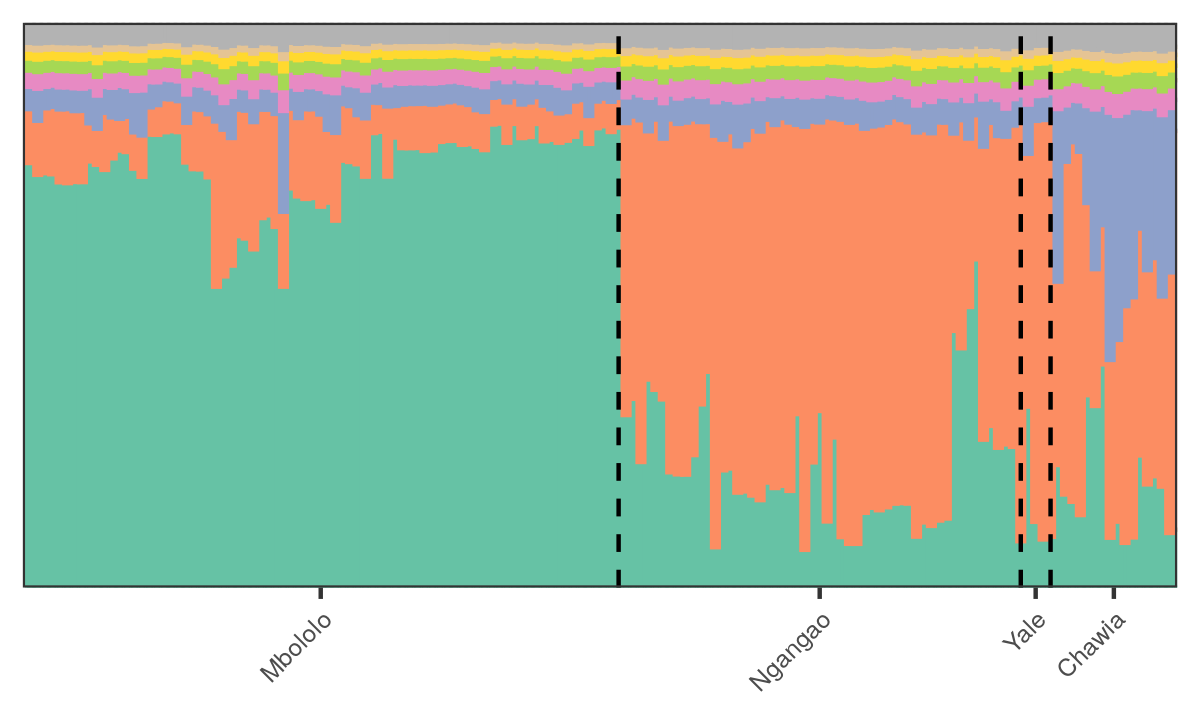
\includegraphics[width=0.980\linewidth,height=0.588\linewidth]{figure/stru_init_fit-1} 

}

\caption[The inferred individual admixtures at $\alpha = 3$]{The inferred individual admixtures at $\alpha = 3$. 
    Each vertical strip is an individual and each color
    a latent population.
    Lengths of colored segments represent the inferred admixture proportions.
    Mbololo, Ngangao, Yale, and Chawia refer to
    geographic regions from which each individual was collected. 
    In the text, we refer to the green, orange, and purple latent populations 
    as population 1, 2, and 3, respectively. }\label{fig:stru_init_fit}
\end{figure}


\end{knitrout}


\subsubsection*{Sensitivity: expected number of populations}

We start by evaluating the sensitivity of the expected number of populations
to the $\alpha$ parameter in the $\betadist{\nu_{nk}\vert 1, \alpha}$ stick distribution. 
We focus on the in-sample quantity. 
Define the expected number of populations as
\begin{align*}
\gpop(\eta; t)
&= \expect{\q(\z\vert\eta)}{\sum_{k=1}^\kmax \ind{ 
\sum_{n=1}^{\nindiv}
\sum_{l=1}^{\nloci}
\sum_{i=1}^2
\z_{\n l i \k} > t}}. 
\end{align*}
% 
Here, the integer value $t$ is a threshold, allowing us to count only populations as present if they contain at least $t$ loci. 
When $t = 0$, this $\gpop$ is equivalent to the expected in-sample number of clusters discussed in \secref{results_iris}, except the summation is now over individuals, loci, and chromosomes. 
As before, $\gpop$ at $t = 0$ has a simple closed form expression as a function of the expectations of $\z_{\n l i \k}$.

When $t > 0$, we again resort to Monte Carlo estimates of $\gpop$. 
As discussed in \secref{results_iris}, we use the re-parameterization trick 
which allows us to use fixed draws from a distribution independent of $\eta$ shared across every computation of $\gpop(\eta; t)$ below. 

The expected number of latent populations is sensitive to $\alpha$ (\figref{stru_alpha_nclusters}). 
Without any thresholding ($t = 0$),
the expected number of populations quickly increases as $\alpha$ increases; 
in fact, it saturates at $\kmax = 20$ when $\alpha = 7$. 
This sensitivity is likely due to the fact that the non-thresholded quantity 
is highly dependent on the behavior of small, nearly unoccupied populations;
even though the probability of a single locus belonging to these rare populations is small, the probability that \textit{none} of the $\nindiv \times \nloci \times 2$ observed genotypes belonging to these rare populations is non-negligable.  

This motivates the use of thresholding in the number of clusters. 
We threshold at $t = 20$ and $t = 40$, corresponding to approximately 
$2$ and $4\%$ 
of the total number of loci in the data set, respectively. 
In the refits, these thresholded estimates still vary between two and four
latent populations. 

The linear approximation, computed at $\alpha_0 = 3$,
produces nearly the same expected number of clusters with $t = 0$ as observed by refitting the model.
However, it under-estimated the sensitivity in the thresholded quantities. 
In particular, the linear approximaition failed to predict the reduction to 
two latent populations at $\alpha = 1$. 

    

\begin{knitrout}
\definecolor{shadecolor}{rgb}{0.969, 0.969, 0.969}\color{fgcolor}\begin{figure}[!h]

{\centering 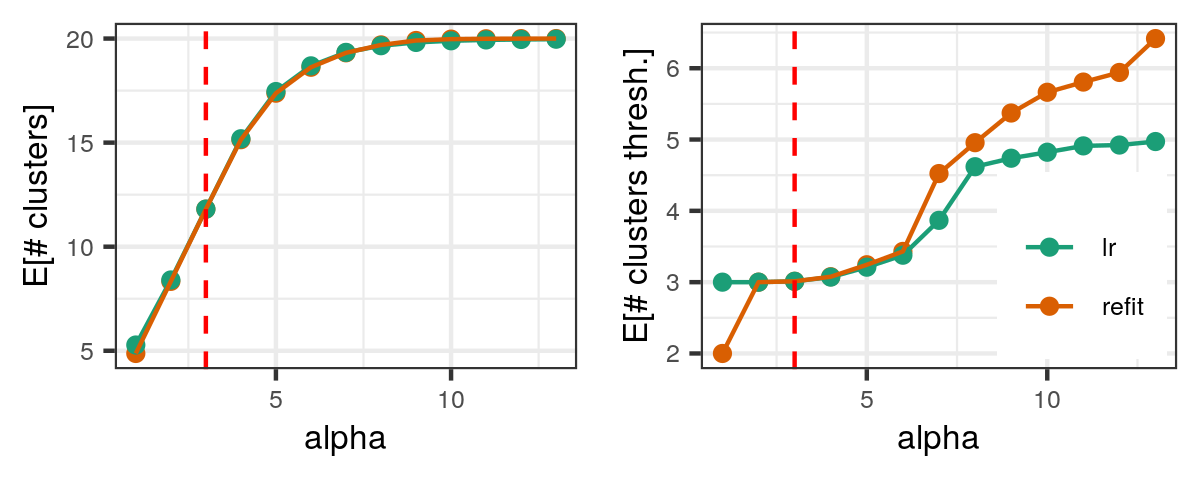
\includegraphics[width=0.980\linewidth,height=0.431\linewidth]{figure/stru_alpha_nclusters-1} 

}

\caption[The expected number of populations in the thrush data as $\alpha$ varies.
    We compute the linear approximation at $\alpha = 3$]{The expected number of populations in the thrush data as $\alpha$ varies.
    We compute the linear approximation at $\alpha = 3$. In the right plot, the threshold is set at $t = 20$ (approximately $1\%$ of loci). }\label{fig:stru_alpha_nclusters}
\end{figure}


\end{knitrout}

We provide some more intuition concerning the expected number of populations with some threshold $t > 0$. 
This posterior quantity is closely related to the expected number of loci belonging to each population, defined as
\begin{align*}
\gloci(\eta; k)
&= \expect{\q(\z\vert\eta)}{\sum_{n=1}^{\nindiv}
\sum_{l=1}^{\nloci}
\sum_{i=1}^2
\z_{\n l i \k}}. 
\end{align*}

\figref{stru_alpha_cluster_weights} plots the expected number of loci belonging to the first six populations, as $\alpha$ varies.
At the initial fit $\alpha = \alpha_0$, there are
1195 expected loci belonging to population1, 
828 belonging to population 2, and 
110 belonging to population 3. 
The remaining populations all have fewer than
12 expected loci. 
Said another way, given a sample of population memberships, 
$\z\sim \q(\z\vert\eta)$, we would expect approximately
$1195$ of
the memberships to belong to population 1, 
$828$ to belong to population 2, and so forth. 
At $\alpha = \alpha_0$, the expected number of loci belonging to 
populations 1, 2, 3 clearly are clearly above either threshold, $t = 20$ or $t = 40$; the expected allocations to the remaining populations are all well below these thresholds. 
Thus, and $\alpha = \alpha_0$, there are clearly 3 populations under our 
thresholded definition. 

At $\alpha = 7$, the expected number of loci belonging to population 4
and population 5 increases to 
$20.7$, 
and a new population emerges above the threshold at $t = 20$. 
On the other hand, at $\alpha = 1$, 
the expected number of loci belonging to population 3 decreases to 
$6.7$, 
below the thresholds $t = 20$ and $t = 40$. 
Thus, the expected number of latent population with thresholding decreases to two. 
The linear approximation under-estimated this decrease in population 3, and therefore continued to predict three latent populations. 


\begin{knitrout}
\definecolor{shadecolor}{rgb}{0.969, 0.969, 0.969}\color{fgcolor}\begin{figure}[!h]

{\centering 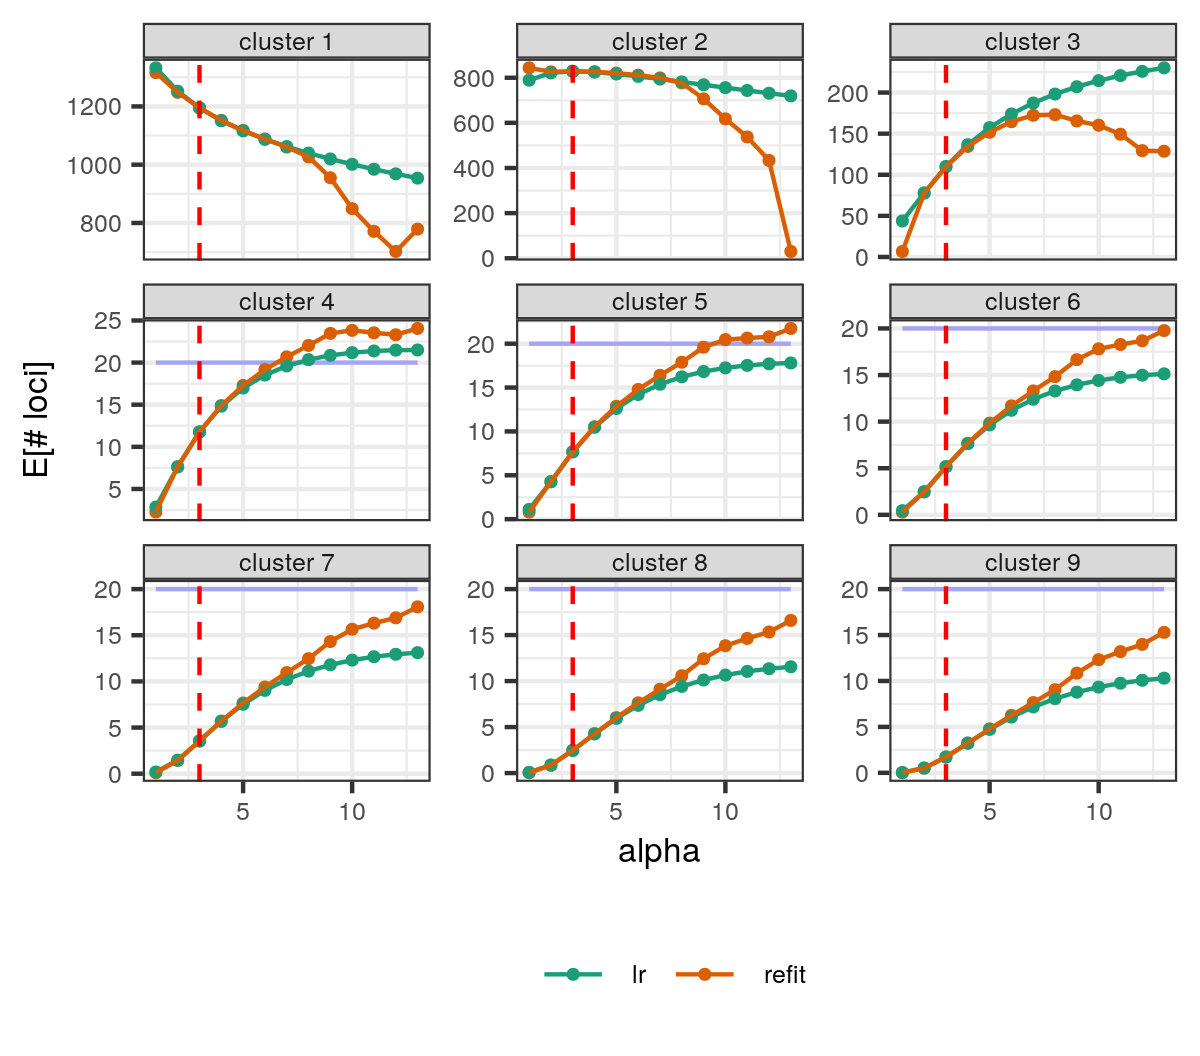
\includegraphics[width=0.980\linewidth,height=0.588\linewidth]{figure/stru_alpha_cluster_weights-1} 

}

\caption{The expected number of loci per cluster as $\alpha$ varies. 
     We compute the linear approximation at $\alpha = 3$. 
     The horizontal blue line corresponds to the threshold in computing the 
    expected number of thresholded clusters in Figure~\ref{fig:stru_alpha_nclusters} }\label{fig:stru_alpha_cluster_weights}
\end{figure}


\end{knitrout}

\subsubsection*{Sensitivity: individual admixtures}

Examining the inferred admixtures in \figref{stru_init_fit} provide clues into historical migration patterns of the genotyped individuals. 
For example, while individuals collected from the Mbololo region are inferred to primarily be admixed with population 1, 
there are a few individuals have abnormally large admixture proportions of population 2 than the rest. 
Conversely, while individuals collected from the Ngangao region are primarily population 2, several individuals have abnormally large admixture proportions of population 1. 
This suggests the presence of migration between the Ngangao and Mbololo regions. 

In this subsection, we evaluate the sensitivity of this conclusion to possible prior perturbations. 
We consider the posterior statistic 
\begin{align*}
\gadmix(\eta; \mathcal{N}, k) = 
 \expect{\q(\z\vert\eta)}{\frac{1}{|\mathcal{N}|}\sum_{n\in\mathcal{N}}
\pi_{\n\k}},
\end{align*}
the average admixture proportion of population $\k$ in a set of 
individuals $\mathcal{N}$. 

We present results on three variations of $\gadmix$: 
the six individuals from the Mbololo region with outlying proportions 
of population 2 ($\mathcal{N} = \{25, ..., 30\}, k = 2$); 
the four individuals from the Ngangao region with outlying proportions 
of population 1 ($\mathcal{N} = \{44, ..., 37\}, k = 1$); 
and all individuals from the Chawia region 
($\mathcal{N} = \{44, ..., 37\}, k = 3$). 
The first two cases are related to the question of migration between the Mbololo and Ngangao regions. 
In the last case, we are examining the sensitivity of the presense of the third population in the Chawia region. 





\begin{knitrout}
\definecolor{shadecolor}{rgb}{0.969, 0.969, 0.969}\color{fgcolor}\begin{figure}[!h]

{\centering 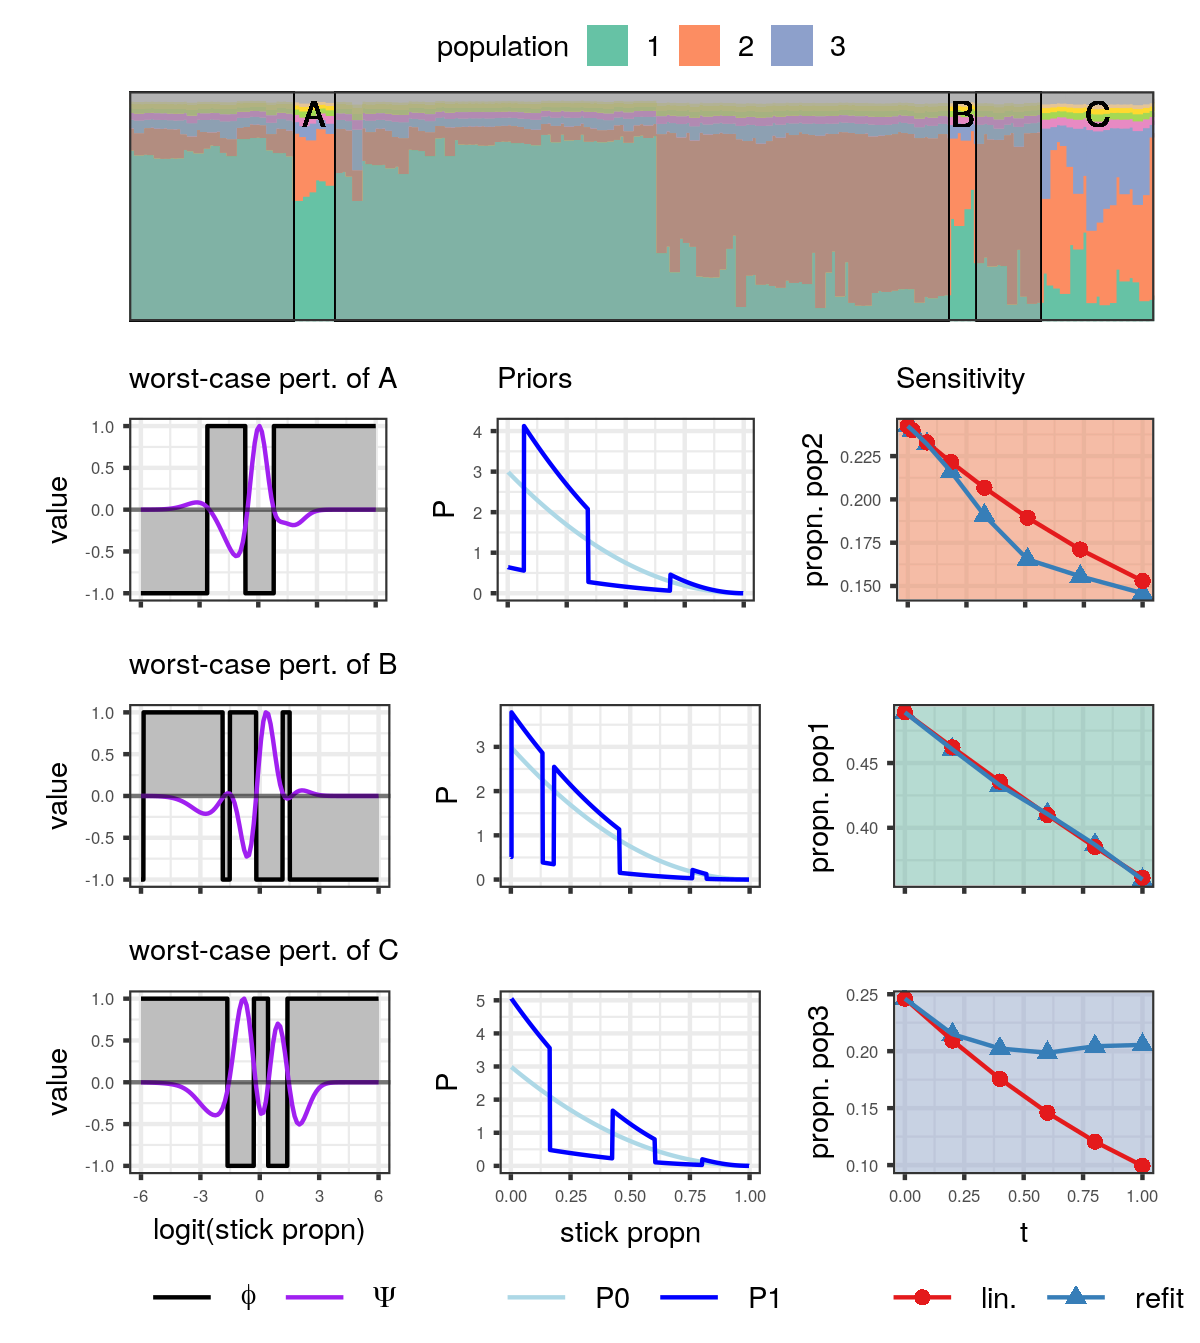
\includegraphics[width=0.980\linewidth,height=1.098\linewidth]{figure/stru_func_sens-1} 

}

\caption[Sensitivity of inferred admixtures for several outlying individuals]{Sensitivity of inferred admixtures for several outlying individuals. 
     For individuals A, 
     we examine the sensitivity of the inferred mixture proportion of the orange
     population.
     For individuals B, 
     we examine the inferred green proportion.
     For the individuals C, we examine the inferred purple proportion.
     (Left column) The worst-case $L_\infty$ negative perturbation in grey,
     plotted against the prior-weighted influence function
     (scaled to have $L_\infty$ norm equal to 1). 
    (Middle column) The effect of this perturbation on the prior density. 
    (Right column) Effects on the inferred admixture. }\label{fig:stru_func_sens}
\end{figure}


\end{knitrout}


\begin{table}[tb]
\centering
\caption{Compute time of results on the structure dataset. }
\begin{tabular}{|r|r|}
\hline 
    & time (seconds) \\ 
    \hline 
    Initial fit & 7 \\
    \hline
    Hessian solve for $\alpha$ sensitivity & 
        0.32\\
    Linear approx. $\eta^{lin}(\alpha)$ for $\alpha = 1, ..., 10$ & 
        0.0059\\
    Refits $\eta(\alpha)$ for $\alpha = 1, ..., 10$ & 
        34\\
    \hline
    The influence function & 0.59\\
    Hessian solve for worst-case $\phi$ &
        0.38\\
    Linear approx. $\eta^{lin}(\epsilon)|_{\epsilon = 1}$ 
      for worst-case $\phi$ &
        0.00085\\
    Refit $\eta(\epsilon)|_{\epsilon = 1}$ 
      for worst-case $\phi$ &
        13\\
    \hline
\end{tabular}
\end{table}

\subsection{Limitations}


\begin{knitrout}
\definecolor{shadecolor}{rgb}{0.969, 0.969, 0.969}\color{fgcolor}\begin{figure}[!h]

{\centering 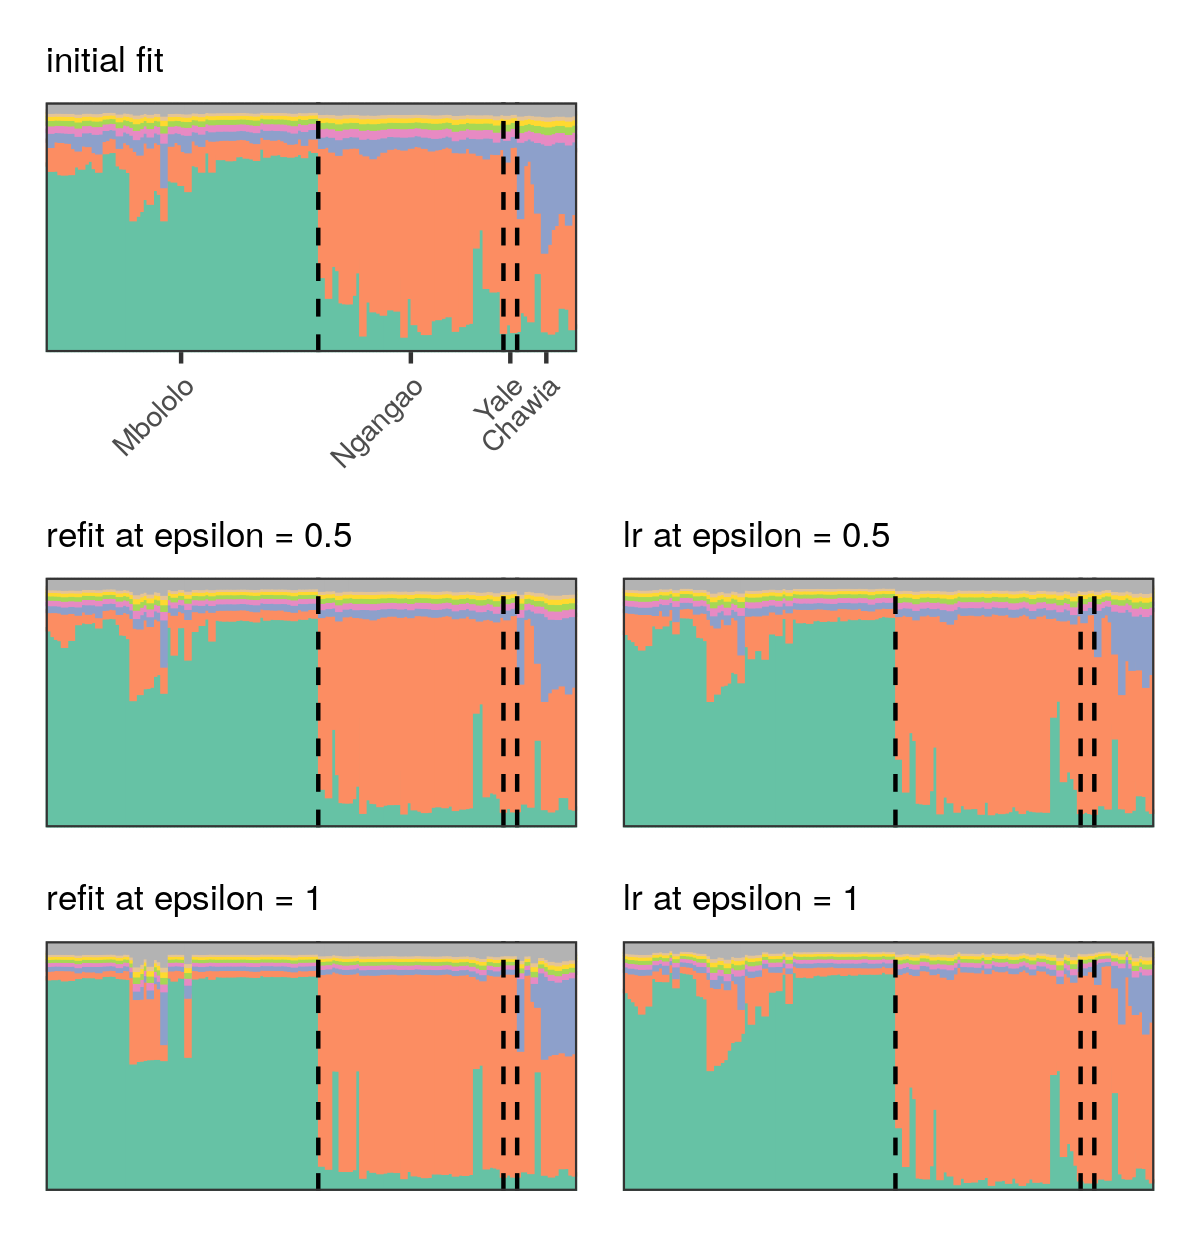
\includegraphics[width=0.980\linewidth,height=0.392\linewidth]{figure/stru_func_sens_admix-1} 

}

\caption{Inferred admixtures after the worst-case prior perturbation 
     to individuals A (second row, Figure~\ref{fig:stru_func_sens}). }\label{fig:stru_func_sens_admix}
\end{figure}


\end{knitrout}



\begin{knitrout}
\definecolor{shadecolor}{rgb}{0.969, 0.969, 0.969}\color{fgcolor}\begin{figure}[!h]

{\centering 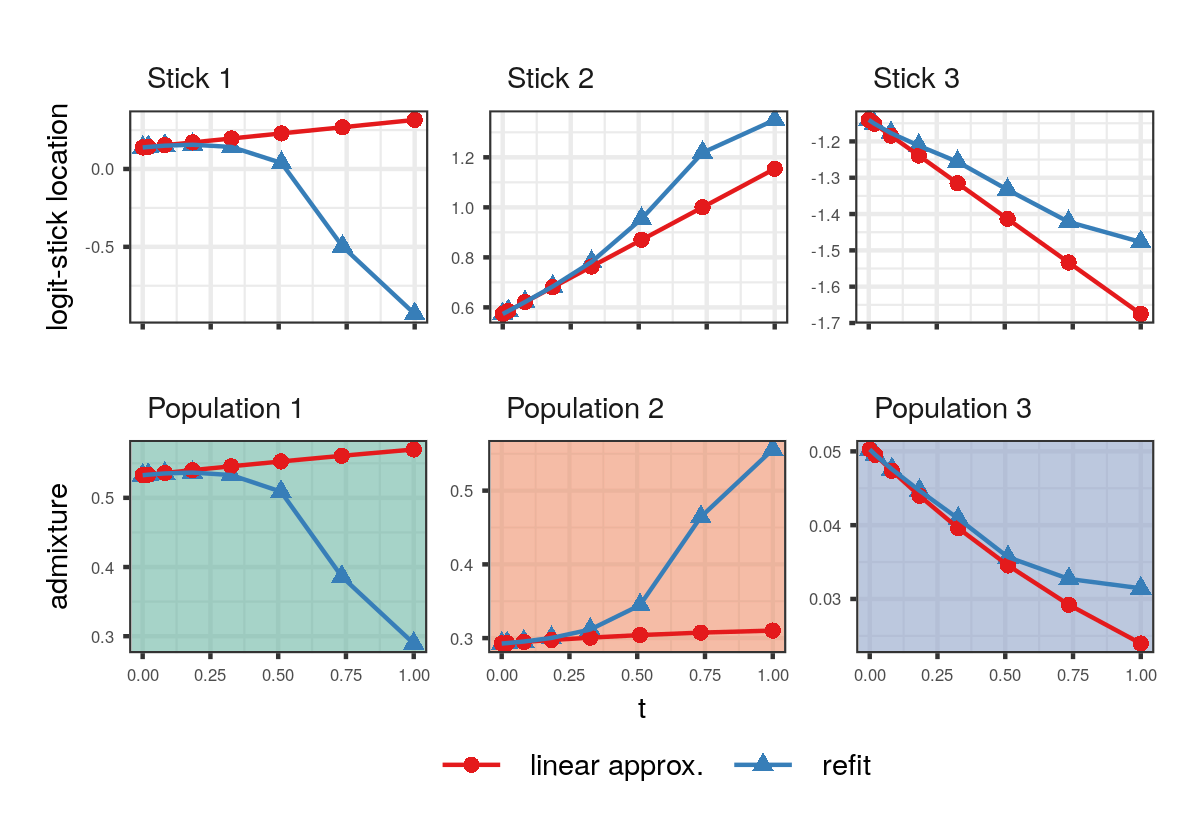
\includegraphics[width=0.980\linewidth,height=0.627\linewidth]{figure/stru_lin_bad_example-1} 

}

\caption[caption]{caption. }\label{fig:stru_lin_bad_example}
\end{figure}


\end{knitrout}


\begin{knitrout}
\definecolor{shadecolor}{rgb}{0.969, 0.969, 0.969}\color{fgcolor}\begin{figure}[!h]

{\centering 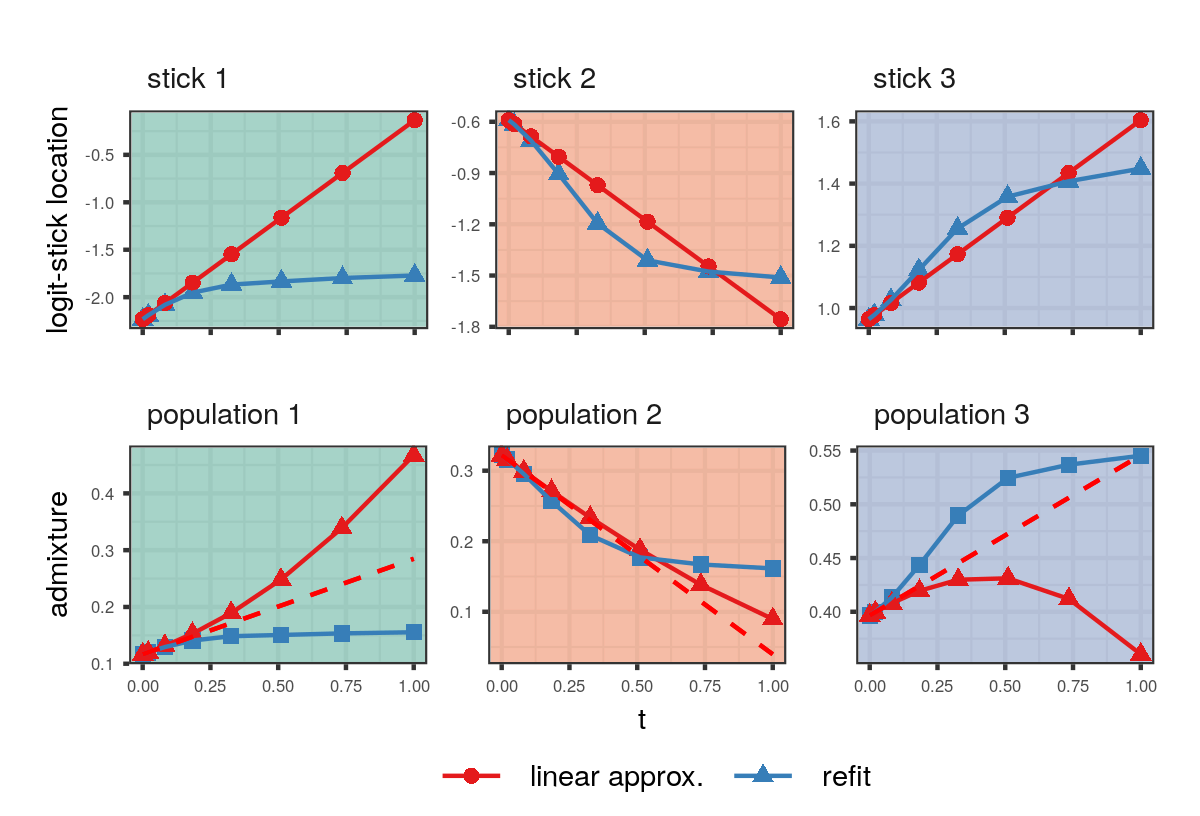
\includegraphics[width=0.980\linewidth,height=0.627\linewidth]{figure/stru_fully_lin_example-1} 

}

\caption[fully linearized good ]{fully linearized good }\label{fig:stru_fully_lin_example}
\end{figure}


\end{knitrout}




